% -*-coding: utf-8;-*-

%\ocgminitext[4cm, bg=red]{Try it here!}{Click the same link or the red mark to close.}
%\ocgminitextlt[bg=black,fg=yellow]{ocg's}{{\color{red}O}ptional {\color{red}C}ontents {\color{red}G}roup}
 \section{Introduction}
\begin{slide}
  \heading{Introduction}
  \begin{wideitemize}
    %\color{dimmed}
  \item <1> When using seasonally unadjusted data, how can we decide what
    is the optimal seasonal adjustment to use?%\pause
    \begin{itemize}
    \item Not theoretical point of view
    \end{itemize}
    
  \item<2> Do we have sensible statistical tools to discriminate among
    the different available alternatives?%\pause
  \item<2> Knowing that the \emph{estimated} components are not
    \emph{observable}, is it enough to pay attention to just the
    component of interest and forget about the remaining ones?%\pause
  \item<2> Is the ideal property of \emph{orthogonality} among the
    different component reasonably fulfilled?
  \item<3> How potential \emph{outliers} and other variants of
    \emph{intervention} analysis affect final estimated components?
  \end{wideitemize}
\end{slide}

\begin{slide}
  \heading{Traditional approach}
  
  \begin{center}
    \LARGE
    \begin{math}
      y_t\;=\;T_t\;+\;C_t\;+\;S_t\;+\;e_t % \varepsilon
    \end{math}
  \end{center}
  
\end{slide}



\section[Exercise]{Small empirical exercise}

\begin{slide}
  \heading{Small empirical exercise} 

  Four monthly time series pertaining to the Spanish economic CLI used
  in: \url{http://uam-ucm-economic-indicators.es/}
  \bigskip
  
  \begin{itemize}
  \item CAR REGISTRATIONS
  \item HOUSING STARTS
  \item CEMENT CONSUMPTION
  \item TRUCKS
  \end{itemize}
  \bigskip

  From 1978M01 to 2013M12
\end{slide}

\begin{slide}
  \heading{Small empirical exercise} 
  \begin{center}
    \resizebox{.93\textwidth}{!}{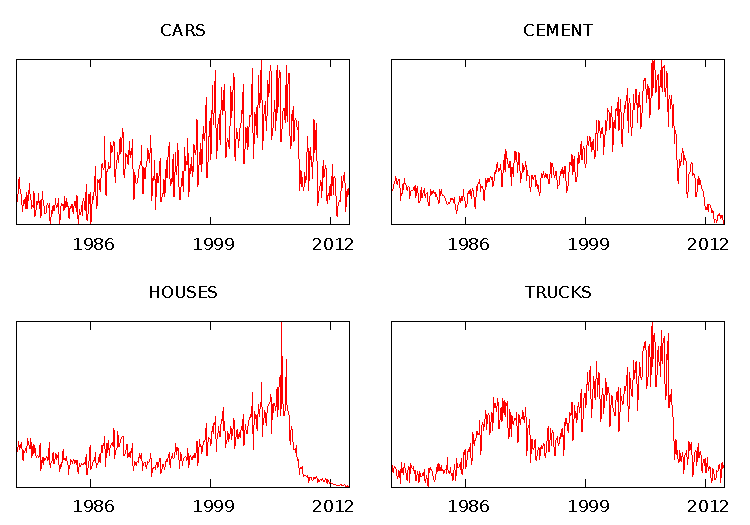
\includegraphics{figuras/4series.pdf}}
  \end{center}
\end{slide}


\section[Methodologies]{Several signal extraction methodologies}

\begin{slide}
  \heading{Several signal extraction methodologies}
  Using several model-based signal extraction methodologies, namely
  \vspace{\stretch{1}}

  \begin{itemize}
  \item SEATS-TRAMO
  \item X-12 ARIMA
  \item Linear Dynamic Harmonic Regression \citep{Bujosa:CSDA-52-999}
  \end{itemize}
  \vspace{\stretch{1}}

  Disclaimer and explanation of the posterior empirical results
\end{slide}

\begin{slide}
  \heading{Dynamic Harmonic Regression Model}

  The {DHR} model consists of several unobserved components plus an
  irregular stationary zero mean component
  $\,{\boldsymbol{e}}=\{e_{t}\}_{t\in\mathbb{Z}}\,$
  \begin{equation}
    \boldsymbol{y}\;=\;\sum_{j=0}^{R}\boldsymbol{s}^{j}\;+\;\boldsymbol{e}.
  \end{equation}
  \begin{itemize}
  \item {DHR} components
    \;$\boldsymbol{s}^{j}\;=\;\{s_{t}^{j}\}_{t\in\mathbb{Z}}\,$\; are
    oscillatory
    \begin{equation}
      s_{t}^{j}\; =\; a_{t}^{j}\cos(\omega_{j}t)+b_{t}^{j}\sin(\omega_{j}t),
    \end{equation}
    where frequency $\omega_{j}$ is associated to the $j$-th component.
  \item Oscillations are modulated by two {\GRW} processes 
    \;$\boldsymbol{a}^{j} = \{a^{j}_t\}_{t\in\mathbb{Z}}$\; and
    \;$\boldsymbol{b}^{j} = \{b^{j}_t\}_{t\in\mathbb{Z}}$.
  \item $\omega_{0}=0$ corresponds to the trend (or zero frequency
    term).
  \item The model is fitted in the frequency domain.
  \end{itemize}
  % are either {RW}
  % processes (and we say that the corresponding {DHR} component,
  % $\boldsymbol{s}^{j}$, follows a RW model) or both are AR(2) processes
  % \emph{with at least one unit root} (when both roots are 1 we say that
  % $\boldsymbol{s}^{j}$ follows an {IRW}; and when one of the roots is
  % less than 1 in absolute value we say $\boldsymbol{s}^{j}$ follows a
  % {SRW}).
  % the
  % other components ($j=1,...,R$) correspond to the seasonal frequency
  % and its harmonics.
\end{slide}

\begin{slide}
  \headingsub{Car registrations Seasonal Factors}{{\color{red} DHR},
    {\color{blue} ST}, {\color{green} X12}}
  \begin{center}
    \resizebox{.93\textwidth}{!}{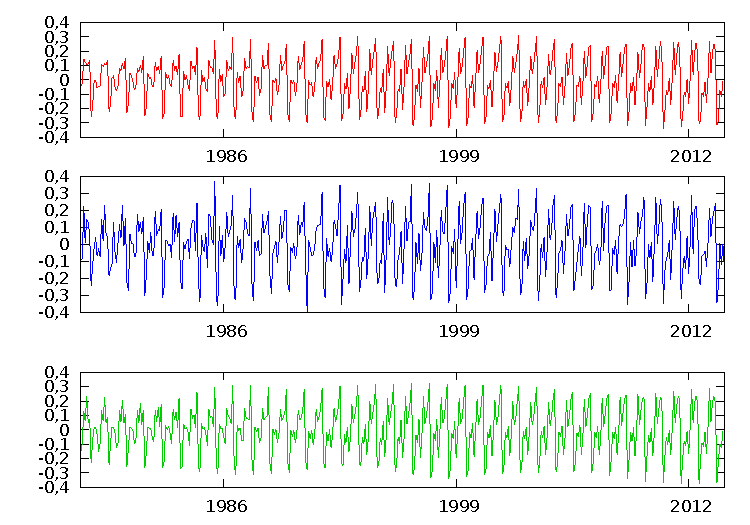
\includegraphics{figuras/CAR_SF.pdf}}
  \end{center}
\end{slide}

\begin{slide}
  \headingsub{Seasonally adjusted Car registrations}{{\color{red}
      DHR}, {\color{blue} ST}, {\color{green} X12}}
  \begin{center}
    \resizebox{.93\textwidth}{!}{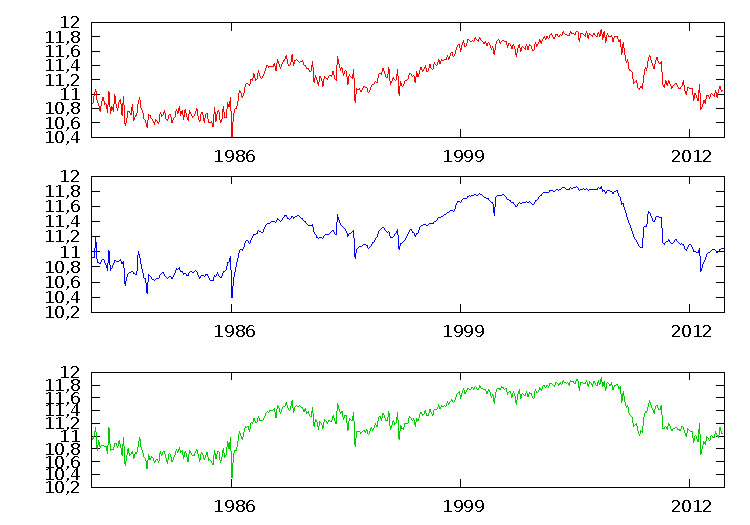
\includegraphics{figuras/CAR_SA.pdf}}
  \end{center}
\end{slide}

\begin{slide}
  \heading{FAC -- First Difference of Seasonally adjusted Car registrations}
  \begin{center}
    \resizebox{.93\textwidth}{!}{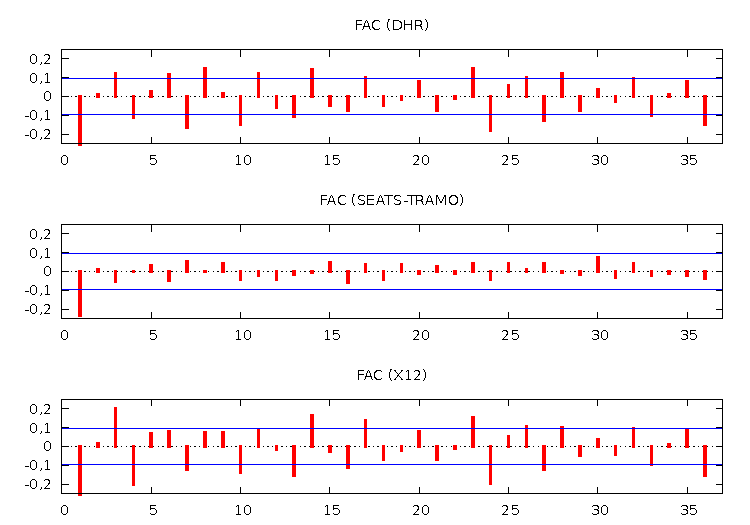
\includegraphics{figuras/fac.pdf}}
  \end{center}
\end{slide}

\begin{slide}
  \heading{Summary of tentative results of the four series}
  \begin{wideitemize}
  \item Outlier detection plus other interventions as easter effects
    and calendar effects are crucial in the estimation of unobserved
    components models
  \item As a matter of fact when you don't use this option in
    SEATS-TRAMO there is evidence of seasonality in the SA
    series
  \item Using outlier detection plus easter and calendar effects
    produce considerable reduction in the estimated residual variances
    ranging from 21\% to 31\%
  \end{wideitemize}
\end{slide}

\section[S\&W data]{Results from a Stock \& Watson data base}

\begin{slide}
  \heading{Results from a Stock \& Watson data base}
  
  \begin{itemize}
  \item Housing starts
  \item IPI
  \item Money supply -- M1
  \item Retail sales
  \end{itemize}
  %Used in Bell's presentation
\end{slide}

\begin{slide}
  \heading{Results from a Stock \& Watson data base}
  \begin{center}
    \resizebox{.93\textwidth}{!}{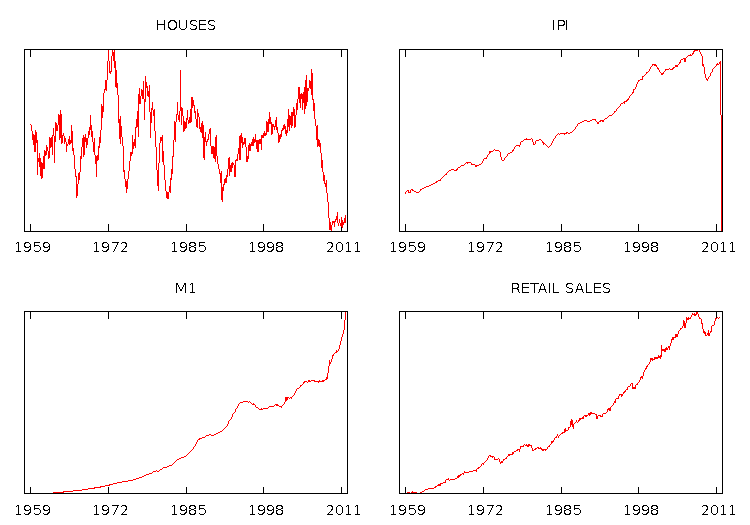
\includegraphics{figuras/4seriesSW.pdf}}
  \end{center}
\end{slide}

\begin{slide}
  \headingsub{Results from a Stock \& Watson data base}{Housing starts}
  \begin{center}
    \resizebox{.93\textwidth}{!}{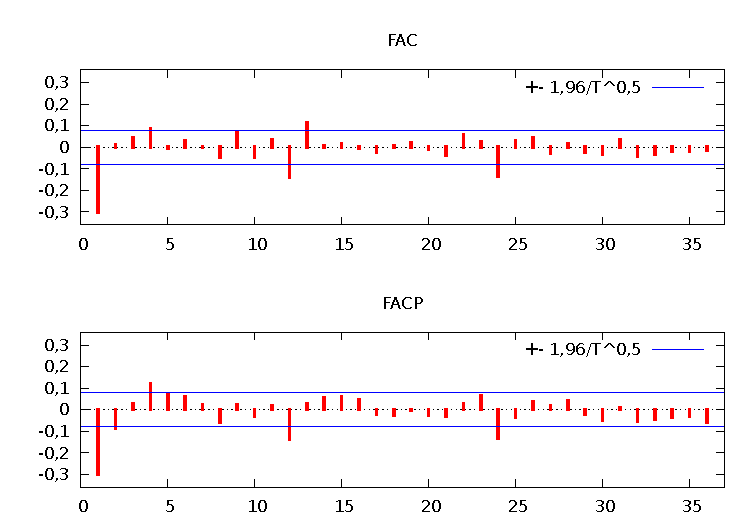
\includegraphics{figuras/corrSW_Houses.pdf}}
  \end{center}
\end{slide}

\begin{slide}
  \headingsub{Results from a Stock \& Watson data base}{IPI}
  \begin{center}
    \resizebox{.93\textwidth}{!}{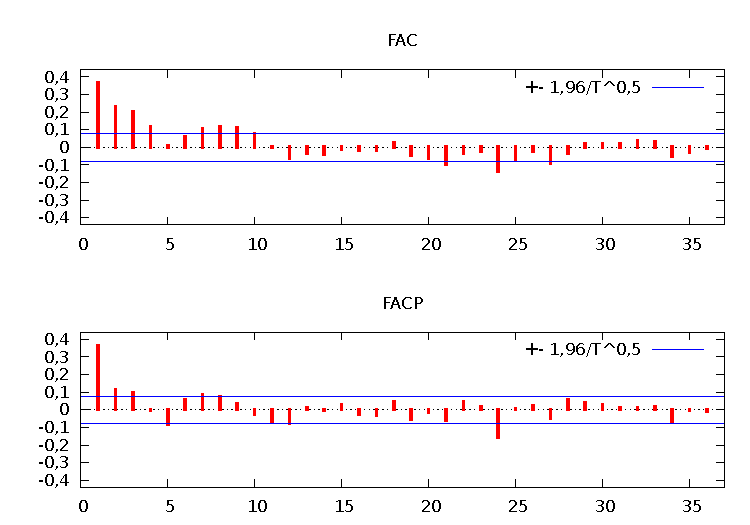
\includegraphics{figuras/corrSW_IPI.pdf}}
  \end{center}
\end{slide}

\begin{slide}
  \headingsub{Results from a Stock \& Watson data base}{Money supply}
  \begin{center}
    \resizebox{.93\textwidth}{!}{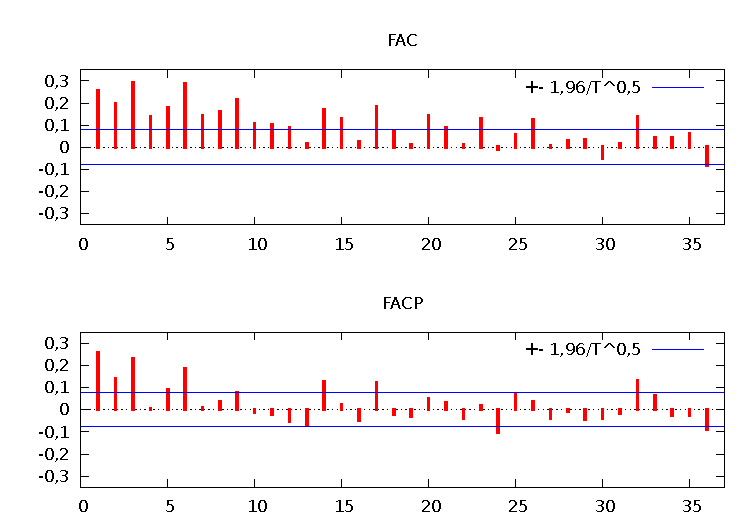
\includegraphics{figuras/corrSW_M1.pdf}}
  \end{center}
\end{slide}

\begin{slide}
  \headingsub{Results from a Stock \& Watson data base}{Retail sales}
  \begin{center}
    \resizebox{.93\textwidth}{!}{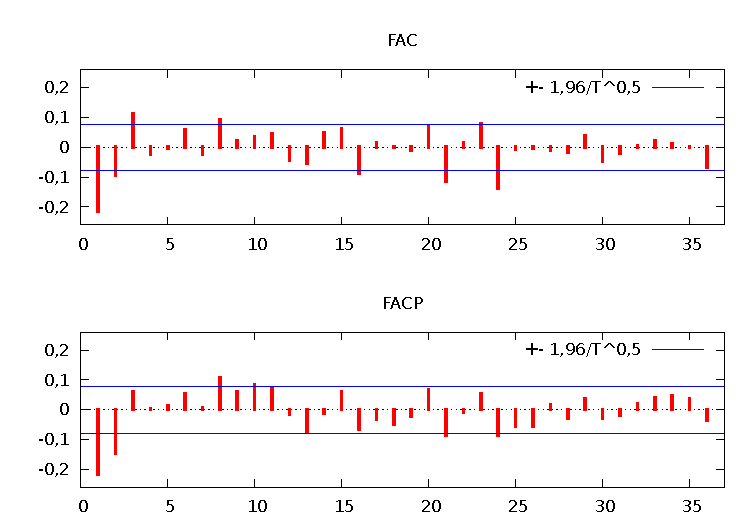
\includegraphics{figuras/corrSW_Sales.pdf}}
  \end{center}
\end{slide}


\section[HP Filter]{Hodrick–Prescott filter}
\begin{slide}
  \heading{Hodrick–Prescott filter}

  \begin{center}
    \large
    \begin{math}
      y_t\ = \tau_t\ + c_t\ + \epsilon_t
    \end{math}
  \end{center}
  Given a positive $\lambda$, there is a trend component $\mathbf{\tau}$ that solves
  \begin{displaymath}
    \min_{\tau}\left(\sum_{t = 1}^T {(y_t - \tau _t )^2 }  + \lambda \sum_{t = 2}^{T - 1} {[(\tau _{t+1}  - \tau _t) - (\tau _t  - \tau _{t - 1} )]^2 }\right)
  \end{displaymath}  
\end{slide}

\begin{slide}
  \heading{Hodrick–Prescott filter}
  \begin{center}
    \resizebox{\fijaAnchura{.98}{.9}}{!}{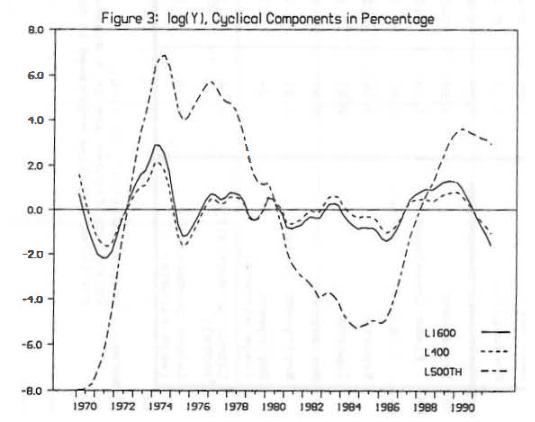
\includegraphics{SinNombre.png}}
  \end{center}
\end{slide}

\section[Climate 1]{The Central England Temperature (CET)}
\begin{slide}
  \heading{The Central England Temperature 1659--2007  (CET)}  
  \begin{center}
    \resizebox{\fijaAnchura{.98}{.8}}{!}{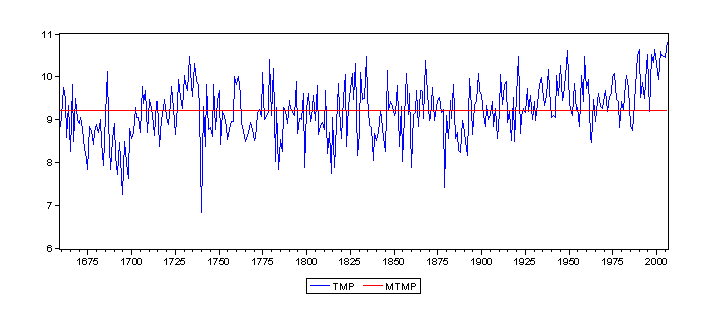
\includegraphics{serie.png}}
  \end{center}
  \vspace{-1.2cm}
  
  \begin{center}
    \resizebox{\fijaAnchura{.98}{.8}}{!}{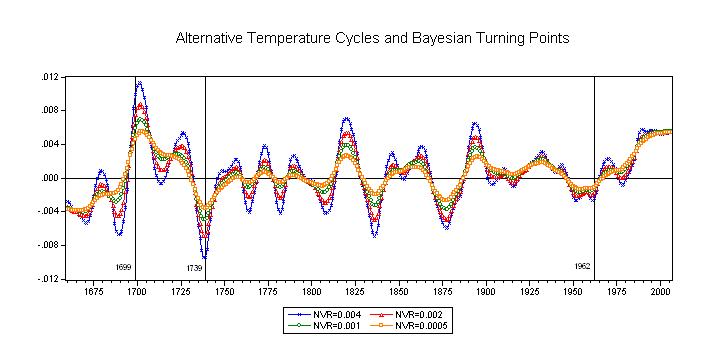
\includegraphics{derivadas.png}}
  \end{center}
\end{slide}

\begin{slide}
  \heading{The Central England Temperature 1659--2023 (CET)}  
  \begin{center}
    %{%\footnotesize SRW trend}\\
    \resizebox{\fijaAnchura{.98}{.97}}{!}{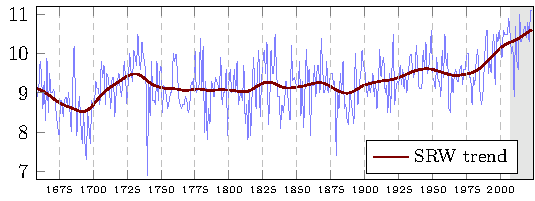
\includegraphics{./figuras/trendSRW.pdf}}\\
    %{%\footnotesize IRW trend}\\
    \resizebox{\fijaAnchura{.98}{.97}}{!}{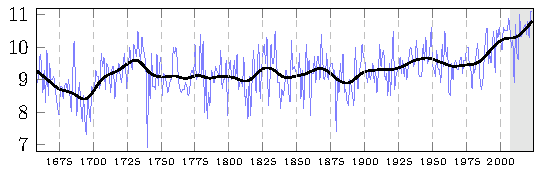
\includegraphics{./figuras/trendIRW.pdf}}
  \end{center} 
\end{slide}

\begin{slide}
  \heading{The Central England Temperature 1659--2023 (CET)}  
  \begin{center}
    %{\footnotesize First difference of SRW trend}\\
    \resizebox{\fijaAnchura{.98}{.97}}{!}{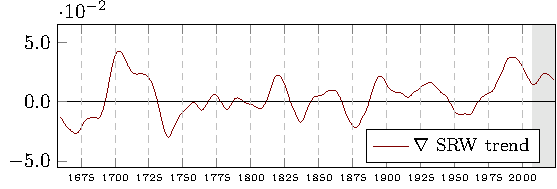
\includegraphics{./figuras/difftrendSRW.pdf}}\\
    %{\footnotesize First difference of IRW trend}\\
    \resizebox{\fijaAnchura{.98}{.97}}{!}{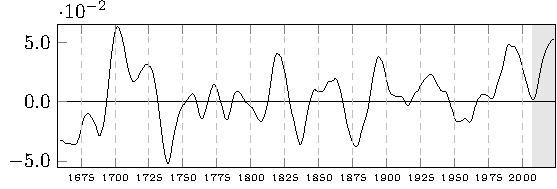
\includegraphics{./figuras/difftrendIRW.pdf}}
  \end{center} 
\end{slide}

% https://unchartedterritory.wordpress.com/2010/03/06/1740-and-all-that/

\section[Climate 2]{Modelling of Global Climate Change}
\begin{slide}
  \heading{Modelling of Global Climate Change}
  \begin{center}
    {\footnotesize Global Temperature Anomaly (\GTA)}\\
    \resizebox{\fijaAnchura{.98}{.97}}{!}{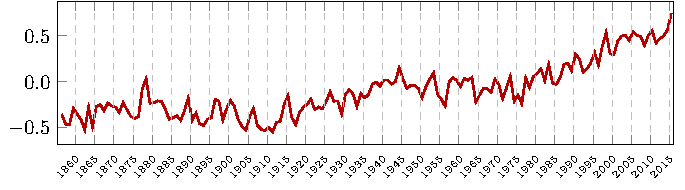
\includegraphics{./figuras/GTA.pdf}}\\
    %{\footnotesize Total Radiative Forcing (\TRF)}\\
    %\resizebox{\fijaAnchura{.98}{.97}}{!}{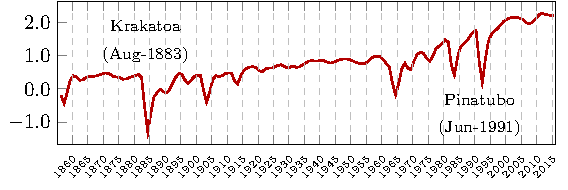
\includegraphics{./figuras/TRF.pdf}}\\
    {\footnotesize Atlantic Multidecadal Oscillation (\AMO)}\\
    \resizebox{\fijaAnchura{.98}{.97}}{!}{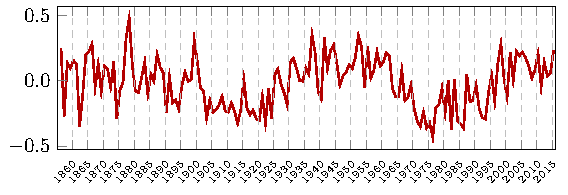
\includegraphics{./figuras/AMO.pdf}}
  \end{center} 
\end{slide}

\begin{slide}
  \heading{Have AMO and GTA a common 63-years cycle?}
  \begin{block}{DHR components for \GTA}
    \centering
    \resizebox{\fijaAnchura{.98}{.75}}{!}{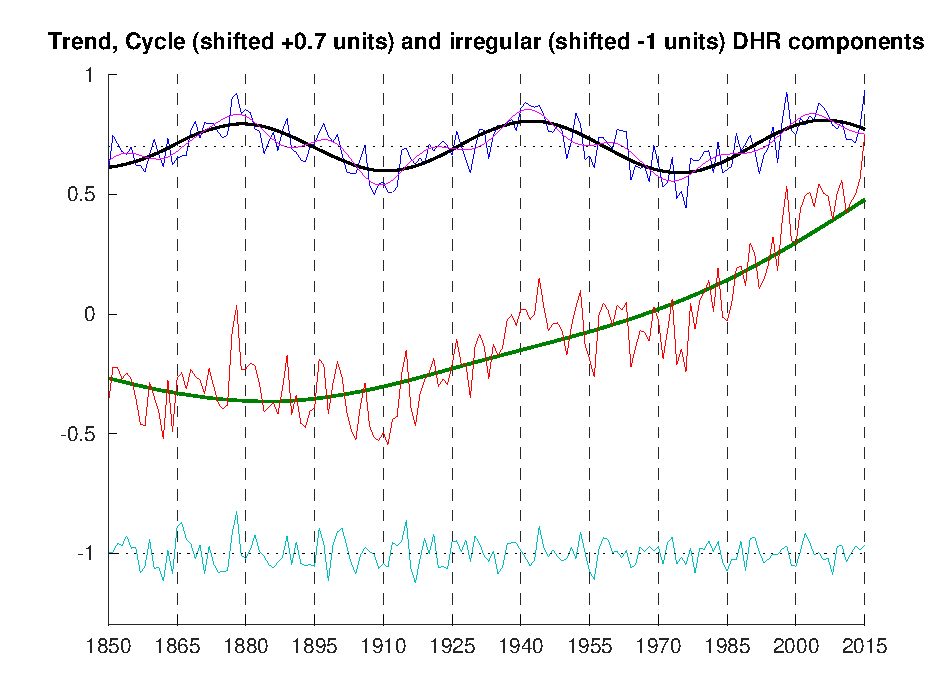
\includegraphics{./figuras/DHRforGTA.pdf}} 
  \begin{displaymath}
    \HLr{GTA}=\HLg{T}+\HLa{S^{\color{black}63}+S^{\color{magenta}21}+\sum ({\color{gray}\text{other harmonics}})}+{\color{teal}Irreg}
  \end{displaymath}
  \end{block}
\end{slide}

\begin{slide}
  \heading{Have AMO and GTA a common 63-years cycle?}
  \begin{block}{DHR Trend-cycle component for \AMO}
    \centering
    \resizebox{\fijaAnchura{.98}{.75}}{!}{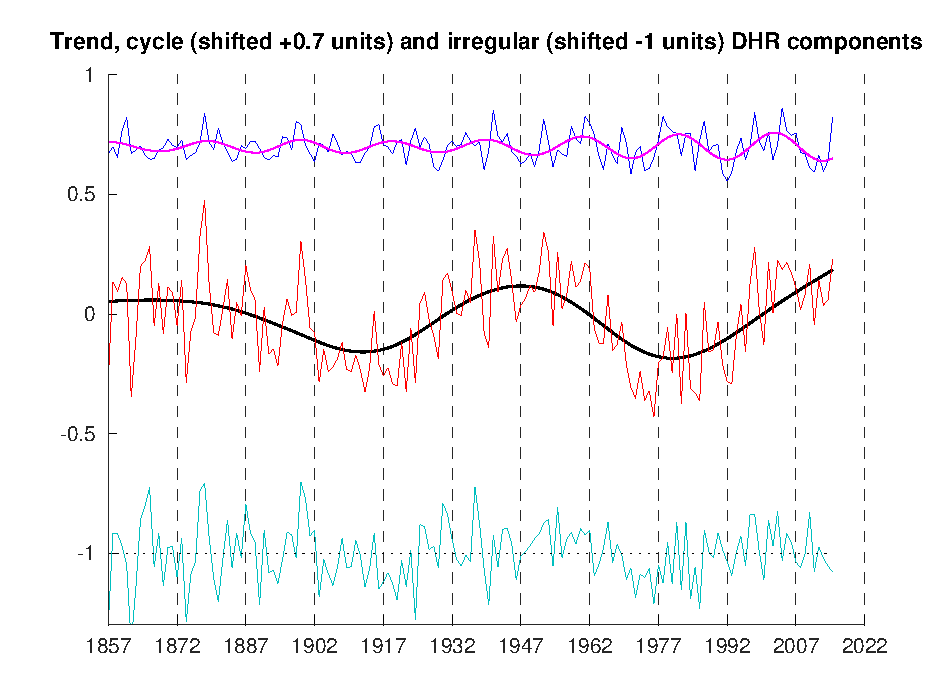
\includegraphics{./figuras/DHRforAMO.pdf}} 
    \begin{displaymath}
      \HLr{AMO}=T+\HLa{S^{\color{magenta}21}+\sum ({\color{gray}\text{other harmonics}})}+{\color{teal}Irreg}
    \end{displaymath}
  \end{block}
\end{slide}


\begin{slide}
  \heading{Have AMO and GTA a common 63-years cycle?}
  \begin{block}{Not clear}
    GTA has a periodic cycle, but not \AMO
    \begin{center}
      \resizebox{\fijaAnchura{.98}{.75}}{!}{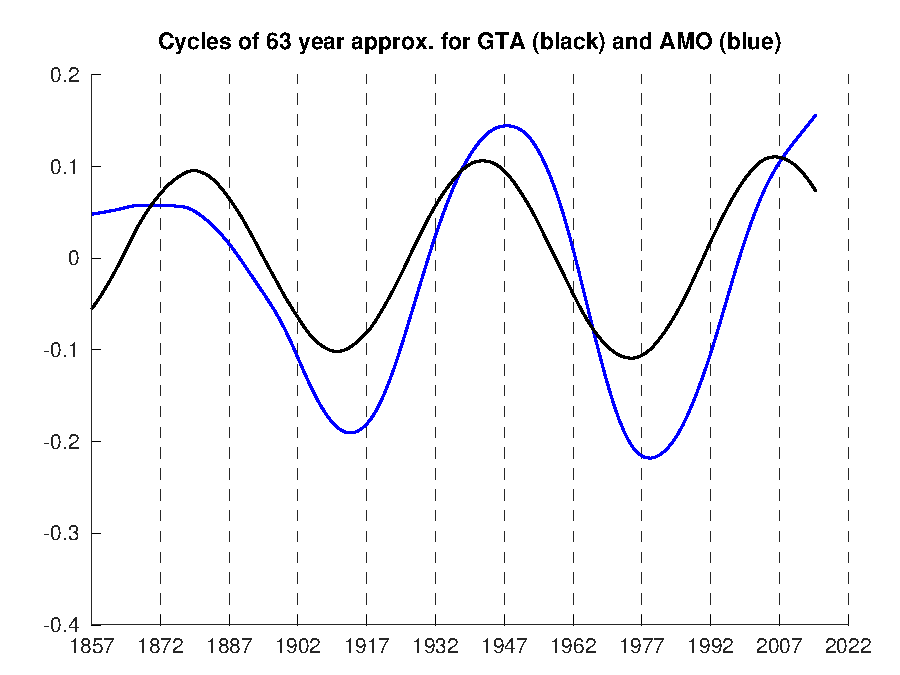
\includegraphics{./figuras/CyclesforGTA&AMO.pdf}}
    \end{center}
  \end{block}
\end{slide}

\begin{slide}
  \heading{Have \HLa{original} AMO and GTA a common 63-years cycle?}
  \begin{block}{DHR components for \emph{``original''} AMO data}
    \centering
    \resizebox{\fijaAnchura{.98}{.75}}{!}{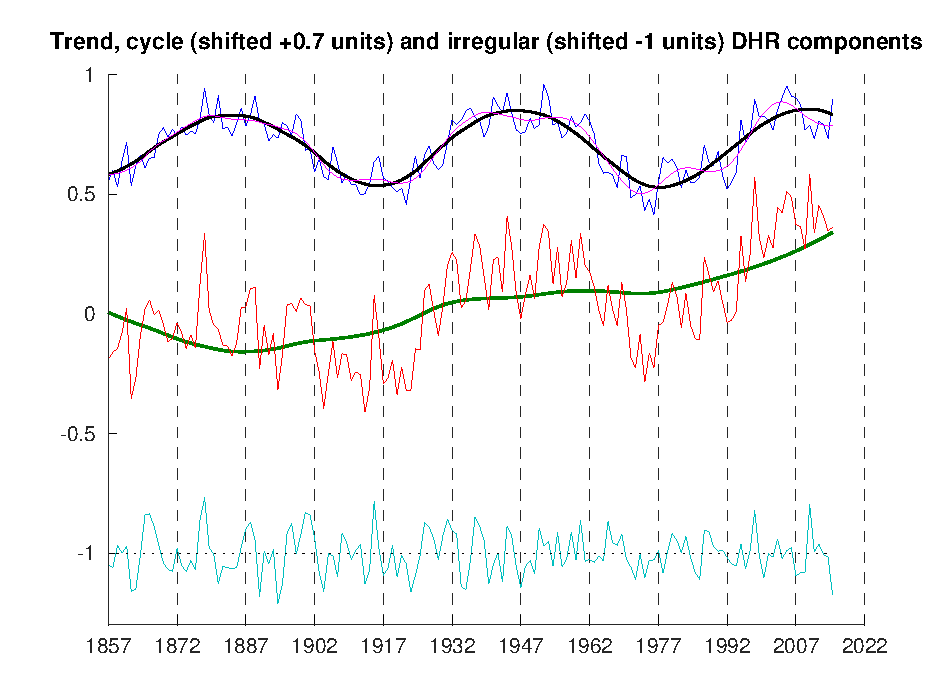
\includegraphics{./figuras/DHRforAMOT.pdf}} 
  \begin{displaymath}
    \HLr{AMO_{\text{with trend}}}=\HLg{T}+\HLa{S^{\color{black}63}+S^{\color{magenta}21}+\sum ({\color{gray}\text{other harmonics}})}+{\color{teal}Irreg}
  \end{displaymath}
  \end{block}
\end{slide}

\begin{slide}
  \heading{Have the \emph{\HLa{``original''}} AMO and GTA a common cycle?}
  \begin{block}{They seem to have a common cycle}
    (as suggested in Professor Young's article)
    \begin{center}
      \resizebox{\fijaAnchura{.98}{.75}}{!}{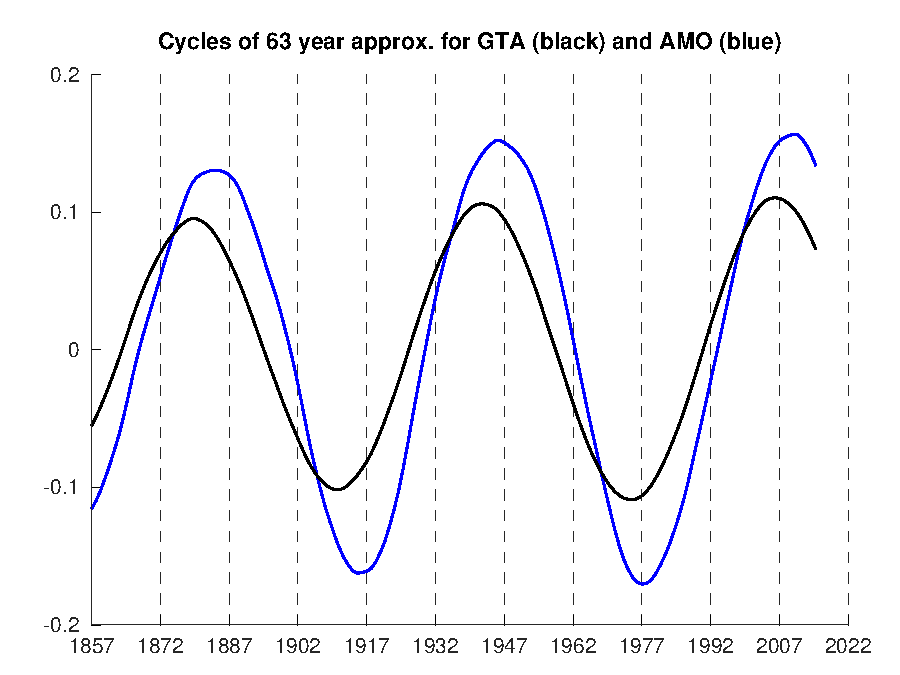
\includegraphics{./figuras/CyclesforGTA&AMOT.pdf}} 
    \end{center}
  \end{block}
\end{slide}


\section[Covid]{Covid 19}
\begin{slide}
  \heading{Number of confirmed cases at 3/22/2020}
  \begin{center}
    \resizebox{\fijaAnchura{.98}{.99}}{!}{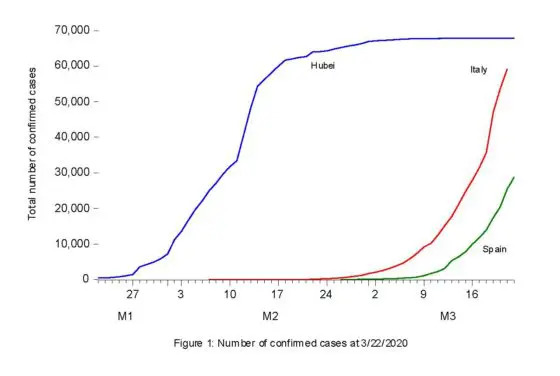
\includegraphics{./figuras/Fig1-560x376.jpg}} 
  \end{center}
\end{slide}

\begin{slide}
  \heading{Observed contagions and forecasts in Spain}
  \begin{center}
    \resizebox{\fijaAnchura{.98}{.99}}{!}{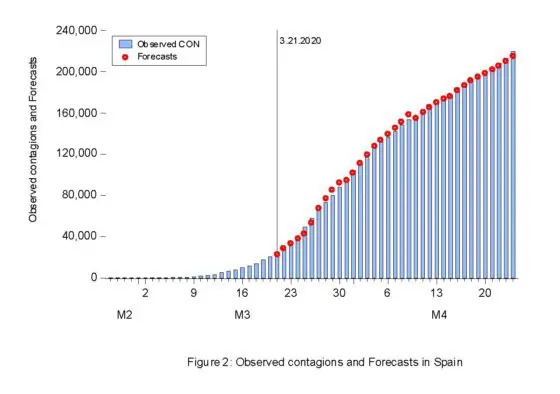
\includegraphics{./figuras/Fig2-560x394.jpg}} 
  \end{center}
\end{slide}

\begin{slide}
  \heading{Observed deaths and forecasts in Spain}
  \begin{center}
    \resizebox{\fijaAnchura{.98}{.99}}{!}{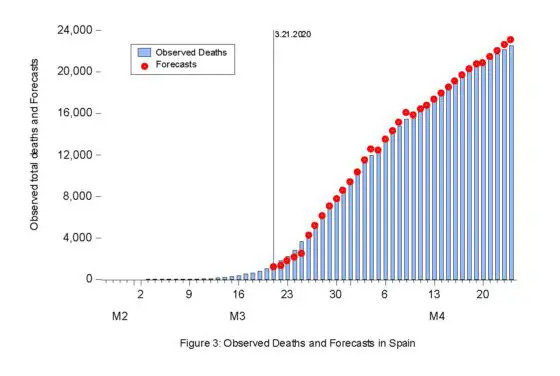
\includegraphics{./figuras/Fig3-560x376.jpg}} 
  \end{center}
\end{slide}


% \section[CET]{Mean Central England Temperature}
% \begin{slide}
%   \heading{Mean Central England Temperature (Degrees Celsius)}
%   \begin{center}
%     Decidir qúe meter aquí
%   \end{center} 
% \end{slide}


\bibliography{referencias/referencias}
\bibliographystyle{referencias/IJF-URL}

\endinput

